\documentclass[12pt, titlepage]{article}

\usepackage{booktabs}
\usepackage{tabularx}
\usepackage{graphicx}
\usepackage{float}
\usepackage{hyperref}
\hypersetup{
    colorlinks,
    citecolor=black,
    filecolor=black,
    linkcolor=red,
    urlcolor=blue
}
\usepackage[round]{natbib}

%% Comments

\usepackage{color}

\newif\ifcomments\commentstrue %displays comments
%\newif\ifcomments\commentsfalse %so that comments do not display

\ifcomments
\newcommand{\authornote}[3]{\textcolor{#1}{[#3 ---#2]}}
\newcommand{\todo}[1]{\textcolor{red}{[TODO: #1]}}
\else
\newcommand{\authornote}[3]{}
\newcommand{\todo}[1]{}
\fi

\newcommand{\wss}[1]{\authornote{blue}{SS}{#1}} 
\newcommand{\plt}[1]{\authornote{magenta}{TPLT}{#1}} %For explanation of the template
\newcommand{\an}[1]{\authornote{cyan}{Author}{#1}}

%% Common Parts

\newcommand{\progname}{Housemates} % PUT YOUR PROGRAM NAME HERE
\newcommand{\authname}{Team \#9, Housemates
\\ Justin Dang - dangj15 
\\ Harris Hamid - hamidh1
\\ Fady Morcos - morcof2 
\\ Rizwan Ahsan - ahsanm7
\\ Sheikh Afsar - afsars} % AUTHOR NAMES                  

\usepackage{hyperref}
    \hypersetup{colorlinks=true, linkcolor=blue, citecolor=blue, filecolor=blue,
                urlcolor=blue, unicode=false}
    \urlstyle{same}
                                


\begin{document}

\title{Verification and Validation Report: \progname} 
\author{\authname}
\date{March 6, 2024}
	
\maketitle

\pagenumbering{roman}

\section{Revision History}

\begin{tabularx}{\textwidth}{p{3cm}p{2cm}X}
\toprule {\bf Date} & {\bf Version} & {\bf Notes}\\
\midrule
March 6 & 1.0 & Version for Rev 0\\
\bottomrule
\end{tabularx}

~\newpage

\section{Symbols, Abbreviations and Acronyms}

\renewcommand{\arraystretch}{1.2}
\begin{tabular}{l l} 
  \toprule		
  \textbf{symbol} & \textbf{description}\\
  \midrule 
  API & Application Programming Interface\\
  P & Pass\\
  F & Fail\\
  \bottomrule
\end{tabular}\\

% \wss{symbols, abbreviations or acronyms -- you can reference the SRS tables if needed}

\newpage

\tableofcontents

\listoftables %if appropriate

\listoffigures %if appropriate

\newpage

\pagenumbering{arabic}

\section{Purpose}

This document describes the results of \href{https://github.com/DangJustin/CapstoneProject/blob/main/docs/VnVPlan/VnVPlan.pdf}{verification and validation plan} that was created earlier on in the software lifecycle of \progname{}. The purpose of this verification and validation  is \begin{enumerate}
    \item Ensure that the requirements listed in the SRS for the Housemates application are correct.
    \item Ensure that the design of the Housemates application satisfies the requirements listed in the SRS.
    \item Ensure the usability of the Housemates application for its prospective users.
\end{enumerate}

To find the the details of each test look at the \href{https://github.com/DangJustin/CapstoneProject/blob/main/docs/VnVPlan/VnVPlan.pdf}{VnV Plan} and search for the associated test id.

\section{Functional Requirements Evaluation}

\subsection{System Tests}

The details of the system tests can be found in section 3.1 of the \href{https://github.com/DangJustin/CapstoneProject/blob/main/docs/VnVPlan/VnVPlan.pdf}{VnV Plan}.

\subsubsection{Bill Management}

\begin{table}[H]
\centering
\begin{tabular}{|c|c|c|}
\hline
Test ID & P & F\\
\hline 
test-BM1-1/2-1 & $\times$ & \\
test-BM3-1 & $\times$ & \\
test-BM4-1 & $\times$ & \\
test-BM5-1 & $\times$ & \\
test-BM6-1 & $\times$ & \\
test-BM7-1 & $\times$ & \\
\hline
\end{tabular}
\caption{\bf Bill Management System Tests}
\end{table}

All bill management system tasks passed as expected.

% \begin{enumerate}

% \item{test-BM1-1/2-1}
					
% Initial State: The bill management system is active and ready to handle events the user provides.
					
% Input: Total amount incurred and users who to split among.
					
% Expected Output: A bill is generated with provided total amount being split evenly among housemates.

% Actual Output: f

% Result: f
					
% \item{test-BM3-1}

					
% Initial State: The bill management system is active and ready to handle events the user provides.
					
% Input: User selects to edit any past expense, alters previously inputted information as deemed fit and may change the users by adding or removing users. 
					
% Expected Output: A new bill is generated with provided total amount being split evenly among housemates Note: this alteration will not change the date on which this expense was incurred.

% Actual Output: f

% Result: f

% \item{test-BM4-1}

					
% Initial State: The bill management system is active and ready to handle events the user provides.
					
% Input: Select from a pre-defined set of categories to assign the type of bill and other necessary inputs.
					
% Expected Output: A bill is generated with provided total amount being split evenly among housemates along with the nature(type) of the bill.

% Actual Output: f

% Result: f

% \item{test-BM5.1/7.1}
		
% Initial State: The bill management system is active and ready to handle events the user provides.
					
% Input: User selects to view any past expense. 
					
% Output: A bill is shown with status of each user who incurred the expense of whether they have paid or received the amount.

% Actual Output: f

% Result: f

% \item{test-BM6.1}
					
% Initial State: The bill management system is active and ready to handle events the user provides.
					
% Input: User selects option to add attachment and adds total amount with users who to split among.
					
% Expected Output: A bill is shown with the total amount split evenly amongst users and an accessible attachment in form of an image as proof of purchase.

% Actual Output: f

% Result: f

% \end{enumerate}

\subsubsection{Task Management}

\begin{table}[H]
\centering
\begin{tabular}{|c|c|c|}
\hline
Test ID & P & F\\
\hline 
test-TM1-1 & $\times$ & \\
test-TM2-1 & $\times$ & \\
test-TM3-1 & $\times$ & \\
test-TM4-1 & $\times$ & \\
test-TM5-1 & $\times$ & \\
\hline
\end{tabular}
\caption{\bf Task Management System Tests}
\end{table}

All task management system tasks passed as expected.

% \begin{enumerate}

% \item{test-TM1-1}
					
% Initial State: Housemates app is open.
					
% Input: Tap on the tasks icon.
					
% Expected Output: User is taken to the Task Management page.

% Actual Output: User is taken to the task management page.

% Result: Pass
					

% \item{test-TM2-1}
					
% Initial State: Task Management page is open.
					
% Input: None.
					
% Expected Output: User can clearly identify their assigned tasks.

% Actual Output: User can clearly see which tasks they're assigned to.

% Result: Pass

% \item{test-TM3-1}
					
% Initial State: Task Management page is open.
					
% Input: Task Name: "Clean the Living Room"
% Due Date: Due Date: 2024-4-05
					
% Expected Output: New task "Clean the Living Room" is added to the list of tasks.

% Actual Output: The task "Clean the Living Room" can be seen when user checks list of tasks.

% Result: Pass

% \item{test-TM4-1}

% Initial State: Task Management page is open with at least one task.
					
% Input: Task Name: "Take out the garbage".
% Due Date: 2024-4-05
% Roommate Assignment: Fardeen Afsar.
					
% Expected Output: Task is assigned to Fardeen, Fardeen can see task.

% Actual Output: Task is assigned to Fardeen, Fardeen can see tasks when they view task management page.

% Result: Pass

% \item{test-TM5-1}
					
% Initial State: Task Management page is open with at least one task.
					
% Input: Task Name: Select a task from the list of tasks.
% Mark task as completed.
					
% Expected Output: Task is marked as completed and status is updated.

% Actual Output: Task is marked as completed and status is updated.

% Result: Pass

% \end{enumerate}
\subsubsection{Scheduling}

\begin{table}[H]
\centering
\begin{tabular}{|c|c|c|}
\hline
Test ID & P & F\\
\hline 
test-SS1-1 & $\times$ & \\
test-SS2-1 & $\times$ & \\
test-SS3-1 & $\times$ & \\
\hline
\end{tabular}
\caption{\bf Scheduling System Tests}
\end{table}

All scheduling system tasks passed as expected.

% \begin{enumerate}

% \item{test-SS1-1}
					
% Initial State: The app is launched and in the home interface.
					
% Input: Tap on the scheduling icon.
					
% Expected Output: The scheduling page is displayed to the user.

% Actual Output: f

% Result: f


% \item{test-SS2-1}
					
% Initial State: The user is on the scheduling page
					
% Input: The user taps on the button to create new event and fills out the event creation form the necessary description.
					
% Expected Output: A new event is listed in the scheduling page.

% Actual Output: f

% Result: f

% \item{test-SS3-1\\}
					
% Initial State: The user is on the scheduling page that shows the existing events.
					
% Input: User views the calendar within the scheduling system.
					
% Expected Output: The user can clearly distinguish between personal events and shared roommate events on the calendar.

% Actual Output: f

% Result: f.

% \end{enumerate}

\subsubsection{Account}

\begin{table}[H]
\centering
\begin{tabular}{|c|c|c|}
\hline
Test ID & P & F\\
\hline 
test-AS-1-1 & $\times$ & \\
test-AS-1-2 & $\times$ & \\
test-AS-1-3 & $\times$ & \\
test-AS-2 & $\times$ & \\
test-AS-3 & $\times$ & \\
test-AS-4 & $\times$ & \\
test-AS-5 & $\times$ & \\
\hline
\end{tabular}
\caption{\bf Account System Tests}
\end{table}

All account system tasks passed as expected.

% \begin{enumerate}

% \item{test-AS1-1}

% Initial State: The valid user credentials to be input do not exist in the system yet.
					
% Input: User selects create account option, then selects the username field, inputs valid username, then selects password field and inputs valid password.
					
% Expected Output: Interface displays that user creation was successful and the credentials are now in the system.

% Actual Output: f

% Result: f
					
% \item{test-AS1-2}

% Initial State: The valid user already exists in the system.
					
% Input: User selects create account option, then selects the username field, inputs the valid username that is already in the system, then selects password field and inputs valid password.
					
% Expected Output: The system does not create the profile and informs the user that account creation was not successful that username is already taken.

% Actual Output: f

% Result: f

% \item{test-AS1-3}

% Initial State: The invalid user credentials do not exist in the system.
					
% Input: User selects create account option, then selects the username field, inputs all cases of invalid passwords and all cases of invalid usernames that is already in the system, then selects password field and inputs valid password.
					
% Expected Output: The system does not create the profile and informs the user of the credential requirements and that creation was not successful due to invalid credentials.

% Actual Output: f

% Result: f

% \item{test-AS2}


% Initial State: The  user credentials do exist in the system.
					
% Input: User selects login option, then enters user credentials.
					
% Expected Output: The system lets the user login.

% Actual Output: f

% Result: f


% \item{test-AS3}

% Control: Manual

% This test is to ensure that users can update profile details.

% Initial State: User is logged in.
					
% Input: User selects edit profiles option, then enters new user details and saves details.
					
% Expected Output: The system saves new user details.

% Actual Output: f

% Result: f

% \item{test-AS4}

% Control: Manual

% This test is to ensure that users can delete their account.

% Initial State: User is logged in.
					
% Input: User selects delete account option and submits the correct user credentials for that account.
					
% Expected Output: The system should delete that user account.

% Actual Output: f

% Result: f


% \item{test-AS5}


% Initial State: The user account already exists in the system.
					
% Input: User selects the "forget password" option and enters username of an existing user account.
					
% Expected Output: The system sends an email to the email associated with the user account.

% Actual Output: f

% Result: f

% \end{enumerate}

\subsection{Unit Testing}

The details of the unit tests can be found in section 4 of the \href{https://github.com/DangJustin/CapstoneProject/blob/main/docs/VnVPlan/VnVPlan.pdf}{VnV Plan}.

\subsubsection{Automated Testing}

Automated testing was conducted using jest and GitHub actions. Automated testing mainly covers the unit testing of \progname{} and is performed automatically whenever a commit is added to the main branch. The purpose of automated testing of \progname{} is to insure that any changes made to the main branch do not break the overall functionality of \progname{}.

\subsubsection{Bill Management}

\begin{table}[H]
\centering
\begin{tabular}{|c|c|c|}
\hline
Test ID & P & F\\
\hline 
UT-B1 & $\times$ & \\
UT-B2 & $\times$ & \\
UT-B3 & $\times$ & \\
\hline
\end{tabular}
\caption{\bf Bill Management Unit Tests}
\end{table}

All unit tests for bill management module passed as expected.

\subsubsection{Task Management}

\begin{table}[H]
\centering
\begin{tabular}{|c|c|c|}
\hline
Test ID & P & F\\
\hline 
UT-T1 & $\times$ & \\
UT-T2 & $\times$ & \\
UT-T3 & $\times$ & \\
UT-T4 & $\times$ & \\
\hline
\end{tabular}
\caption{\bf Task Management Unit Tests}
\end{table}

All unit tests for task management module passed as expected.

\subsubsection{Scheduling}

\begin{table}[H]
\centering
\begin{tabular}{|c|c|c|}
\hline
Test ID & P & F\\
\hline 
UT-S1 & $\times$ & \\
UT-S2 & $\times$ & \\
UT-S3 & $\times$ & \\
UT-S4 & $\times$ & \\
UT-S5 & $\times$ & \\
\hline
\end{tabular}
\caption{\bf Scheduling Unit Tests}
\end{table}

All unit tests for scheduling module passed as expected.

\subsubsection{Account}

\begin{table}[H]
\centering
\begin{tabular}{|c|c|c|}
\hline
Test ID & P & F\\
\hline 
UT-A1 & $\times$ & \\
UT-A2 & $\times$ & \\
UT-A3 & $\times$ & \\
UT-A4 & $\times$ & \\
\hline
\end{tabular}
\caption{\bf Account Unit Tests}
\end{table}

All unit tests for account module passed as expected.


\section{Nonfunctional Requirements Evaluation}

\subsection{Usability}
The usability of the app was evaluated by conducting a survey with five participants who were asked to complete basic tasks within the app and provide feedback on their experience. This survey can be found in section 5.2 of the \href{https://github.com/DangJustin/CapstoneProject/blob/main/docs/VnVPlan/VnVPlan.pdf}{VnV Plan}. The survey consisted of 13 questions, including multiple-choice, rating scale, and open-ended questions. The main findings from the survey are summarized below along with some key data quantified:

\begin{itemize}
    \item User Profile: All the participants were students who lived with roommates or housemates and often split their bills with other people.
    \item First Impression: None of the participants found the app to be visually appealing, and most of them described it as bland, generic, or unpolished. They also had difficulty locating the main features or functions of the app.
    \item Performance: The participants were generally satisfied with the speed and performance of the app, but some of them encountered errors or bugs while using it, such as not being able to create a user or join a group.
    \item Feedback and Guidance: The app did not provide helpful feedback or guidance when the participants made a mistake or encountered an issue. Most of them did not know what to do when they faced a problem and had to refresh the page or try again.
    \item Difficulty: The participants found some features or functions to be particularly difficult to use or understand, such as joining a group, splitting an expense, or paying off a bill. They also complained about the amount of typing required and the lack of information or options available.
\end{itemize}

\begin{figure}[H]
    \centering
    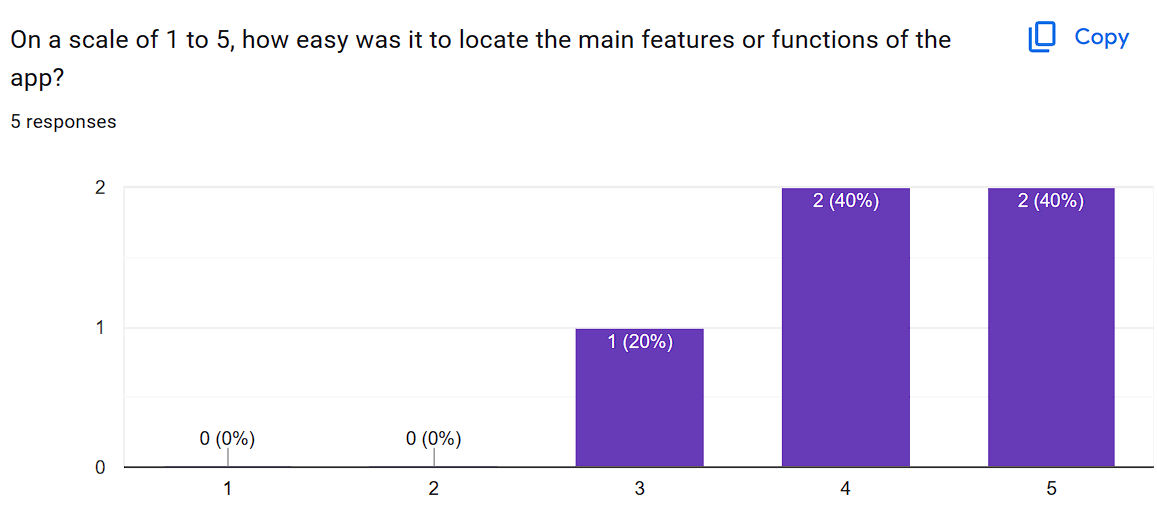
\includegraphics[width=1\linewidth]{Usability_1.png}
    \caption{Ease of locating main features}
    \label{fig: Ease of locating main features}
\end{figure}

\begin{figure}[H]
    \centering
    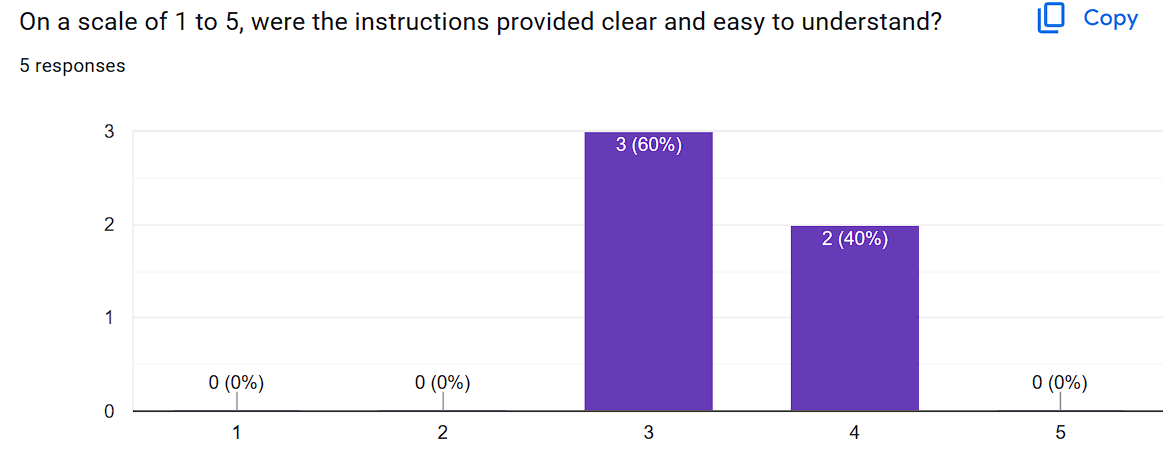
\includegraphics[width=1\linewidth]{Usability_2.png}
    \caption{Clear instructions}
    \label{fig: Clear instructions}
\end{figure}

\begin{figure}[H]
    \centering
    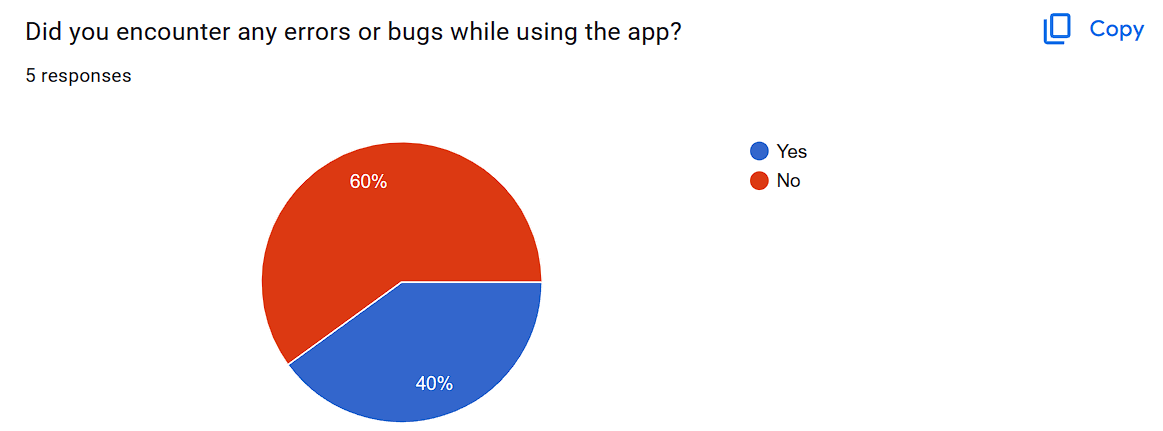
\includegraphics[width=1\linewidth]{Usability_3.png}
    \caption{Bugs encountered}
    \label{fig: Bugs encountered}
\end{figure}

\begin{figure}[H]
    \centering
    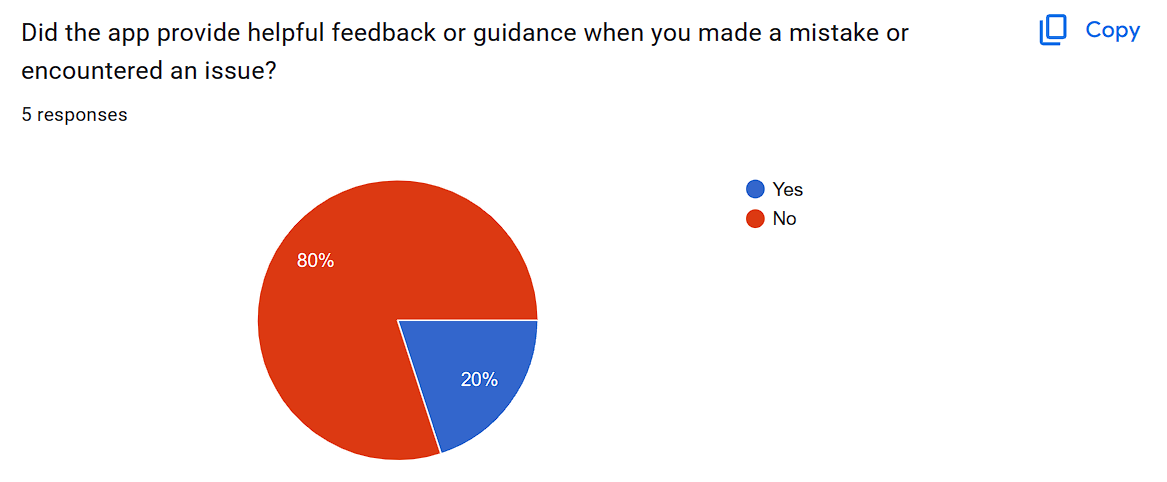
\includegraphics[width=1\linewidth]{Usability_4.png}
    \caption{App feedback to user errors}
    \label{fig: App feedback to user errors}
\end{figure}

\begin{figure}[H]
    \centering
    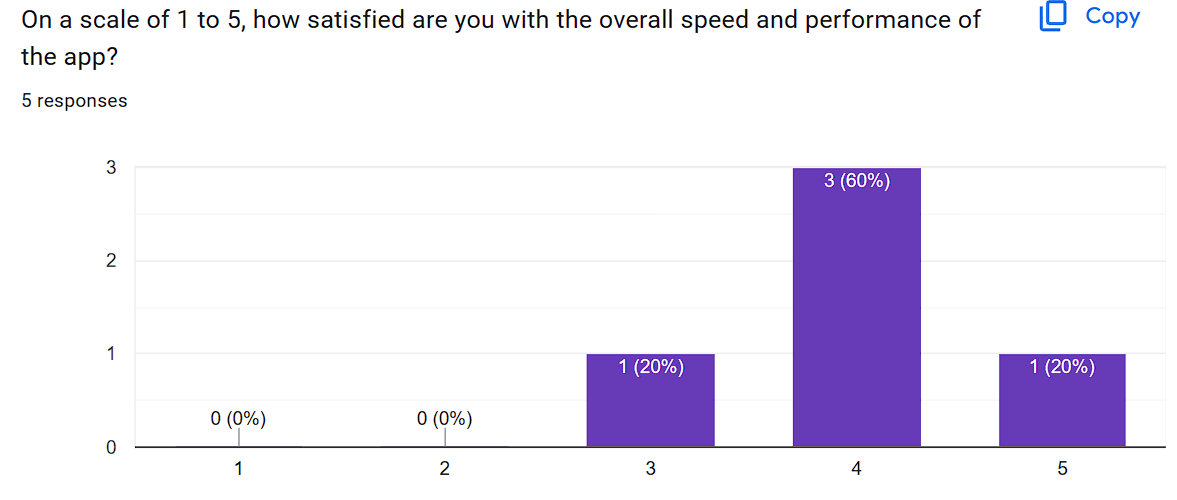
\includegraphics[width=1\linewidth]{Usability_5.png}
    \caption{Performance of app}
    \label{fig: Performance of app}
\end{figure}

\begin{figure}[H]
    \centering
    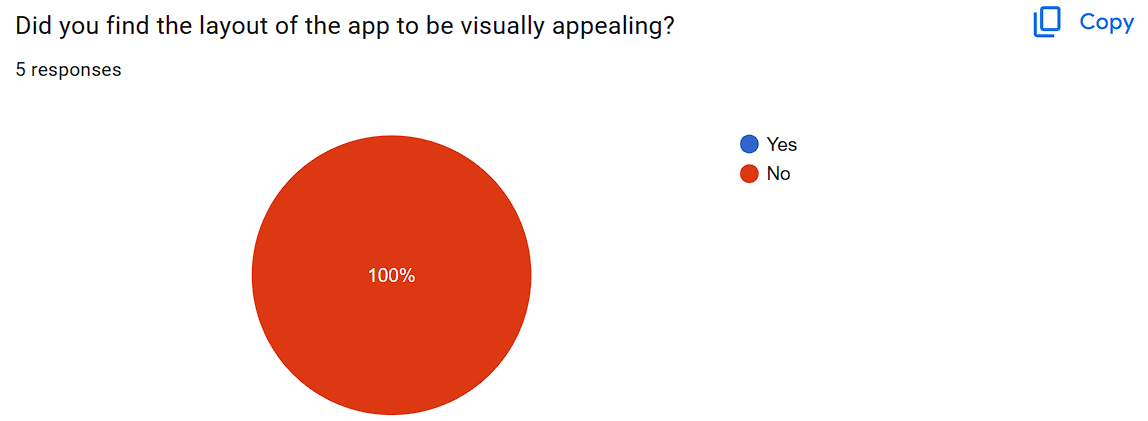
\includegraphics[width=1\linewidth]{Usability_6.png}
    \caption{Visual appeal}
    \label{fig: Visual appeal}
\end{figure}

		
\subsection{Performance}

Performance testing for \progname{} was focused testing the back-end server of the application. This was done using Jmeter, which is a load testing tool that helps analyze the performance of the backend API of \progname{}. The test plan involved creating 100 users for \progname{} and having them make common requests to the backend server API (e.g getting user information after logging in). The results of performance testing can be seen in the graph below.


\begin{figure}[H]
    \centering
    \hspace*{-1cm}
    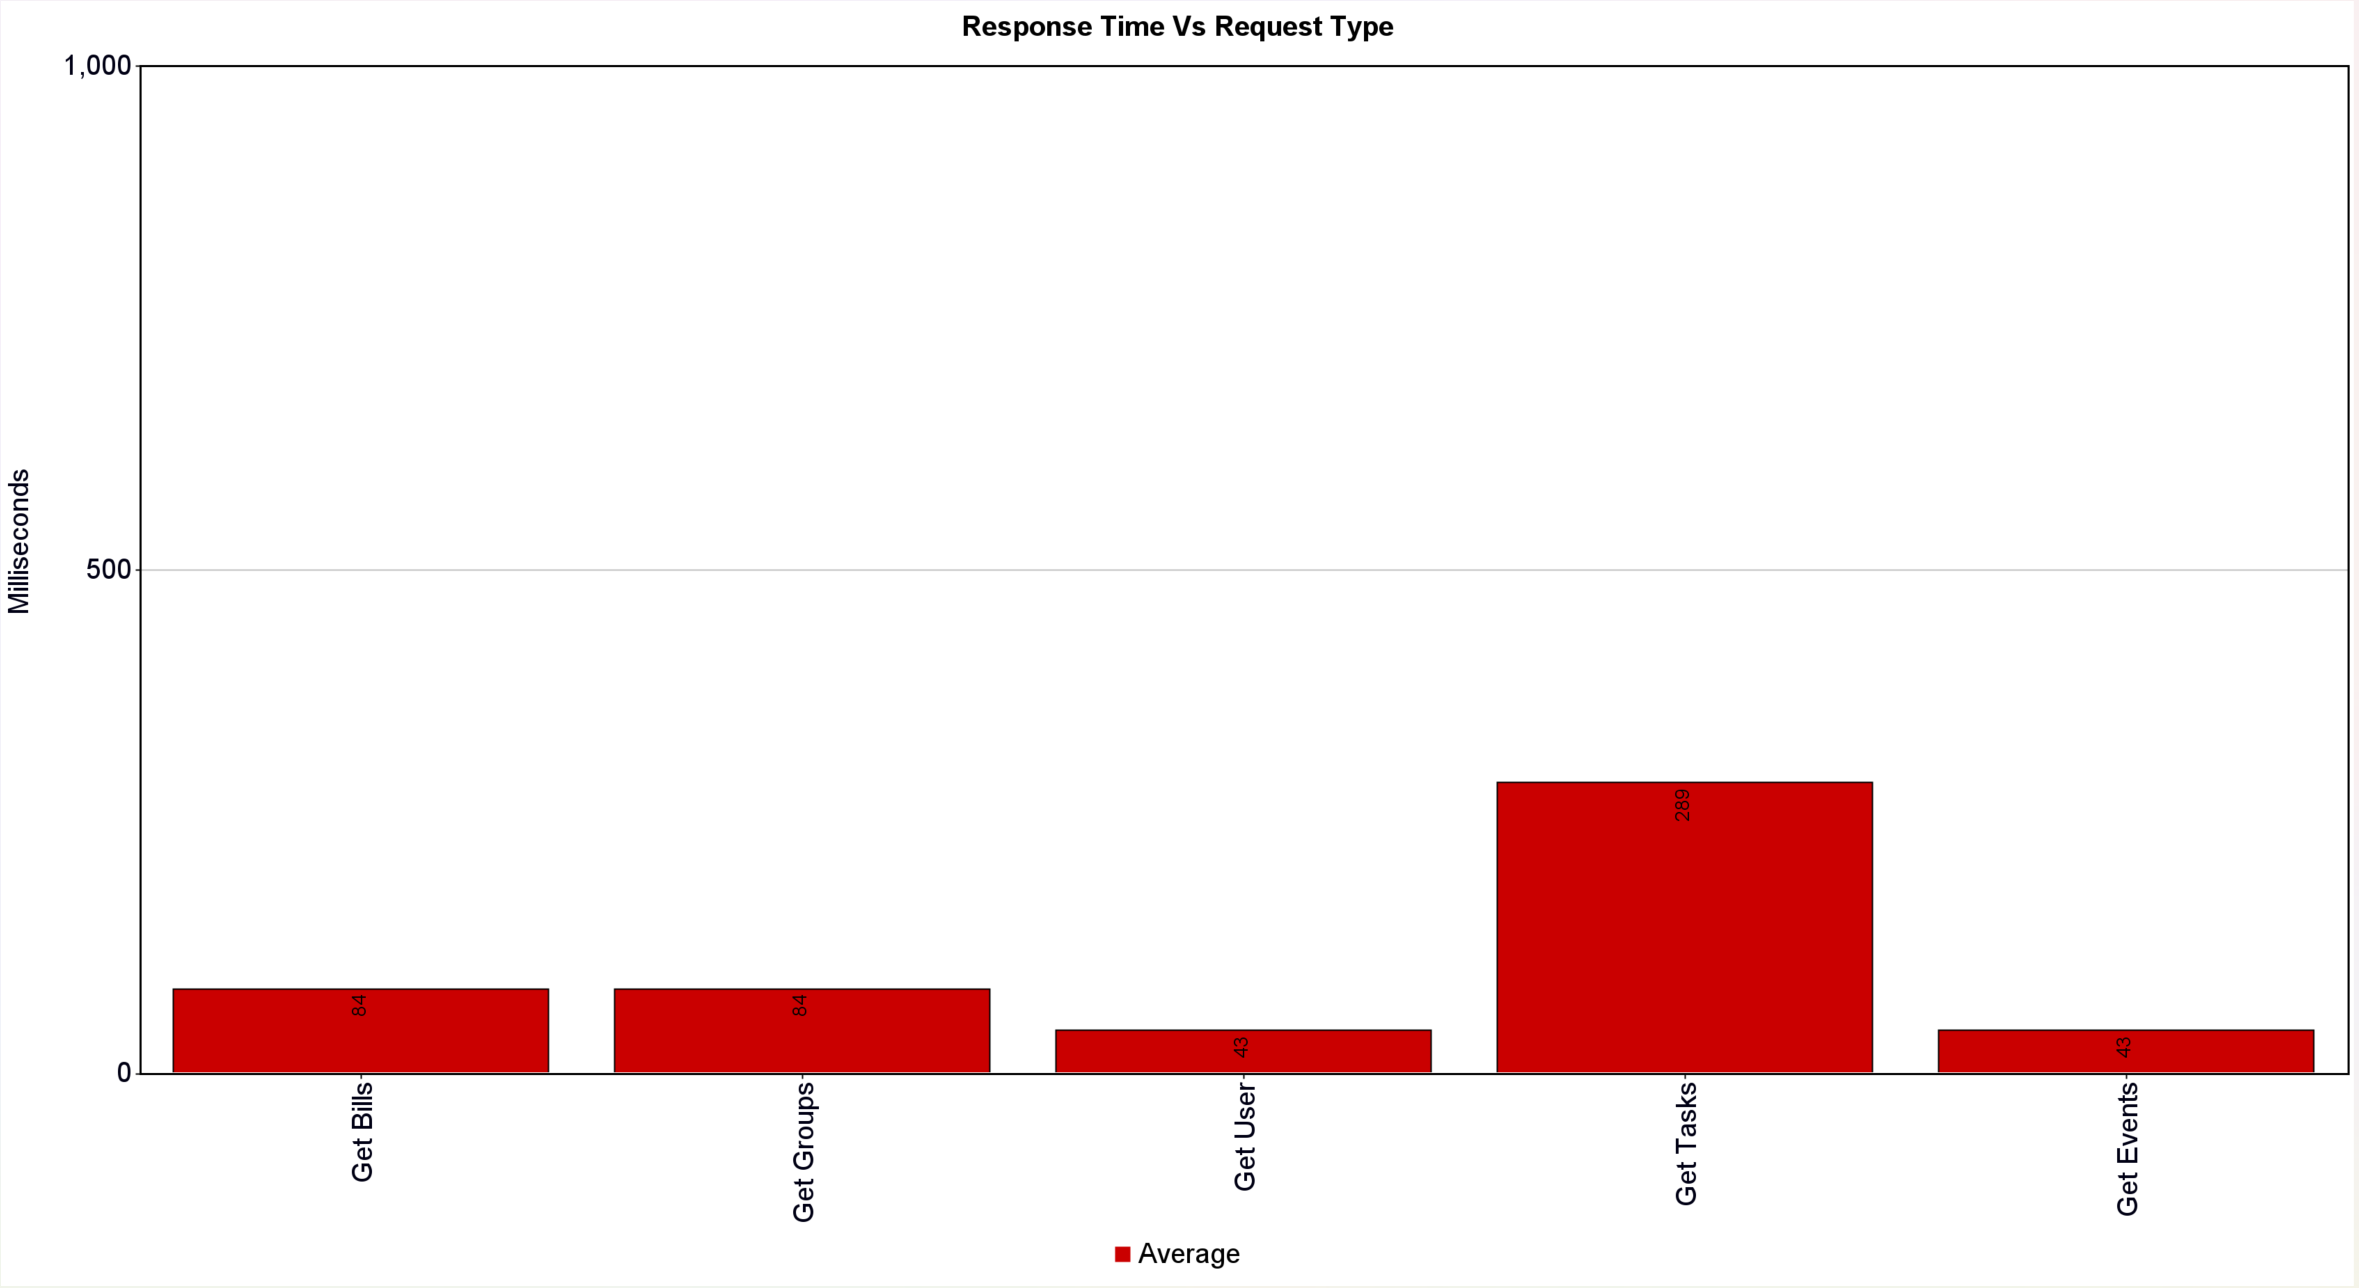
\includegraphics[width=1.25\linewidth]{Response_Time.png}
    \caption{Average Response Times of \progname{} API}
    \label{fig:responsetimegraph}
\end{figure}

As can be seen through the above graph the response times to user requests is quite fast ranging from around  40 - 300 ms. This is fast enough so that there should not be noticeable delay in \progname{} on the user end. As such this indicates to us that \progname{} can handle 100 concurrent users and as a result we concluded that the performance of \progname{} is sufficient for our current purposes. In the future if necessary the database of \progname{} could be upgraded in order to handle more users.


\subsection{Other Non-functional Tests}

The details of these non-functional tests can be found in section 3.2 of the \href{https://github.com/DangJustin/CapstoneProject/blob/main/docs/VnVPlan/VnVPlan.pdf}{VnV Plan}.

\begin{table}[H]
\centering
\begin{tabular}{|c|c|c|}
\hline
Test ID & P & F\\
\hline 
test-LF-A1-1 & & $\times$ \\\
test-LF-A1-2 & & $\times$ \\\
test-UH-E1-1 & $\times$ & \\\
test-UH-E1-2 & $\times$ & \\\
test-UH-P1 & $\times$ & \\\
test-UH-L1-1 & & $\times$ \\\
test-UH-L1-2 & & $\times$ \\\
test-UH-A1 & $\times$ & \\\
test-P-SL1 & $\times$ & \\\
test-P-PA1 & $\times$ & \\\
test-P-RFT1 &  & $\times$ \\
test-P-C1 & $\times$ & \\\
test-OE-PE1 & $\times$ & \\
test-OE-PR1 & & $\times$ \\
test-M-M1 & $\times$ & \\
test-S-A1 & $\times$ & \\
test-S-IN1 & $\times$ & \\
test-S-P1 & $\times$ & \\
test-C-SC1 & $\times$ & \\
\hline
\end{tabular}
\caption{\bf Non-Functional System Tests}
\end{table}

For the non-functional system tests most passed, but some did not. test-OE-PR1 failed because \progname{} isnt available on Google Play Store, test-P-RFT-1 failed because \progname{} doesn't work well offline yet, test-LF-A1-1, test-LF-A1-2, test-UH-L1-1, and test-UH-L1-2 failed because of reasons described in usability section of this VnV report.


% \subsubsection{Look and Feel Requirements}
		
% \begin{enumerate}

% \item{test-LF-A1-1}
					
% Initial State: The application is run on a phone.
					
% Input/Condition: The developers will observe the interface of the application. 
					
% Expected Result: The developers of the application will confirm the interface follows \href{https://m3.material.io/foundations}{Google's material design guidelines}. 
					
% Actual Result: F

% \item{test-LF-A1-2}
					
% Initial State: The application is run on a phone.
					
% Input/Condition: Users will be shown the  application and be asked if it is visually appealing and intuitively designed. 
					
% Output/Result: 90 \% of users will say that the application is visually appealing and intuitively designed. 
					
% Actual Result: F
					
% \end{enumerate}

% \subsubsection{Usability and Humanity Requirements}
		
% \begin{enumerate}

% \item{test-UH-E1-1}

% Initial State: The application is run on a phone.
					
% Input/Condition: The user will be asked to navigate to one of the main features of the application.
					
% Output/Result: The user will be able to navigate to the function within 5 taps.
					
% Actual Result: F

% \item{test-UH-E1-2}
					
% Initial State: The application is run on a phone.
					
% Input/Condition: Users will be shown the application and be asked if it they find the application easy to navigate. 
					
% Output/Result: 90 \% of users will say that the application is easy to navigate. 
					
% Actual Result: F
					
% \item{test-UH-P1}

% Initial State: The application is run on a phone.
					
% Input: The developers will observe the interface of the application.
					
% Output: The developers of the application will observe that the interface is in Canadian English.
					
% Actual Result: Interface is in Candian English

% \item{test-UH-L1-1}

% Initial State: The application is run on a phone.
					
% Input: The user will be given an overview of the application and a walkthrough of a specific feature of the application in 30 minutes. The user will be then asked to use that feature without assistance.
					
% Output: The user will be able to use that feature effectively without external assistance.
					
% Actual Result: F

% \item{test-UH-L1-2}
			
% Initial State: The application is run on a phone.
					
% Input/Condition: Users will be shown the application in a walkthrough and be asked to use it. Afterwards they will be asked if it they found the application easy to learn. 
					
% Output/Result: 90 \% of users will say that the application is easy to learn. 
					
% Actual Result: F

% \item{test-UH-A1}

% Type: Non-functional, Dynamic, Manual 
					
% Initial State: The application is run on a phone.
					
% Input/Condition: The developers will observe the interface of the application. 
					
% Output/Result: The developers of the application will confirm the interface uses \href{https://support.google.com/accessibility/android/answer/6006564?hl=en}{android accessibility features.}
					
% Actual Result: F
					
% \end{enumerate}

% \subsubsection{Performance Requirements}

		
% \begin{enumerate}

% \item{test-P-SL1}
					
% Initial State: The application is run on a phone.
					
% Input/Condition: The developers will observe the interface of the application. 
					
% Output/Result: The developers of the application will go through all of the various pages/interfaces of the application. They will confirm the response time to user input is within 0.5 s for all interactions.

% Actual Result: F

% \item{test-P-PA1}

% Initial State: The application is run on a phone.
					
% Input/Condition: The developers will use the bill-splitting feature of the application. 
					
% Output/Result: The output of the bill-splitting feature will be accurate to two decimal places.
					
% Actual Result: F

% \item{test-P-RFT1}

					
% Initial State: The application is run on a phone.
					
% Input/Condition: The developers will disconnect the phone from the server. They will then attempt to use the features of the application.
					
% Output/Result: The features of the application will continue to work for at least 10 minutes after losing connection.
					
% Actual Result: F

% \item{test-P-C1}

					
% Initial State: The application is run on a phone.
					
% Input/Condition: 100 users will be simulated trying to login to application servers.
					
% Output/Result: The application servers will be able to process those login requests.
					
% Actual Result: pass, See performance section


% \end{enumerate}

% \subsubsection{Operational and Environmental Requirements}

% This section contains the tests for the Operational and Environmental Requirements.
		
% \begin{enumerate}

% \item{test-OE-PE1}
					
% Initial State: The application is run on a phone with Android OS.
					
% Input/Condition: The developers will observe the application on multiple different phones running Android OS.
					
% Output/Result: The application will be able to run.
					
% Actual Result: F
					
% \item{test-OE-PR1}
					
% Initial State: The development of the application is complete.
					
% Input/Condition: The developers will submit the app for the Google Play Store.
					
% Output/Result: The application will be available on the Google Play Store.
					
% Actual Result: Fail, Not available yet

% \end{enumerate}

% \subsubsection{Maintainability and Support Requirements}

		
% \begin{enumerate}

% \item{test-M-M1}
					
% Initial State: The development of the application is complete.
					
% Input/Condition: The developers will check the \href{https://github.com/DangJustin/CapstoneProject}{GitHub}  for the Housemates application.
					
% Output/Result: The documentation for the application will be available under the docs folder.
					
% Actual Result: N/A
					

% \end{enumerate}

% \subsubsection{Security Requirements}

		
% \begin{enumerate}

% \item{test-S-A1\\}
					
% Initial State: The application is run on a phone.
					
% Input/Condition: The developers will try to access one account's user data from another user account.
					
% Output/Result: The user data will not be accessible from other user accounts.
					
% Actual Result: Pass
					
% \item{test-S-IN1}
					
% Initial State: The application is run on a phone.
					
% Input/Condition: The developers will attempt to introduce incorrect data into the input fields of the application.
					
% Output/Result: The application will prevent the incorrect data from being entered into the database.
					
% Actual Result: Pass

% \item{test-S-P1\\}
					
% Initial State: The application is run on a phone.
					
% Input/Condition: The developers will launch the application.
					
% Output/Result: The application will show the information collection policy of the application.
					
% Actual Result: Fail, No information collection policy shown

% \end{enumerate}

% \subsubsection{Compliance Requirements}

		
% \begin{enumerate}

% \item{test-C-SC1\\}
					
% Initial State: The application is run on a phone.
					
% Input/Condition: The developers will observe the application.
					
% Output/Result: The application will follow the \href{https://play.google.com/about/developer-content-policy/}{Google Play development standards}.
					
% Actual Result: F

% \end{enumerate}

	
% \section{Comparison to Existing Implementation}	

% N/A

% This section will not be appropriate for every project.

\section{Conclusions based off VnV Data}

The main area of improvement for \progname{} is in the usability department. As evidenced from the data from the usability survey most users are not satisfied with the current state of the \progname{} application. The non-functional tests that failed also mainly have to do with the usability of \progname{}. As such, the main focus for revision 1 of \progname{} will be on improving the usability of \progname{}. The changes that we plan to implement with revision 1 of the \progname{} application are covered in the next section.


\section{Changes Due to Testing}

% \wss{This section should highlight how feedback from the users and from 
% the supervisor (when one exists) shaped the final product.  In particular 
% the feedback from the Rev 0 demo to the supervisor (or to potential users) 
% should be highlighted.}


\subsection{Planned Changes due to Revision 0 Feedback}

For the Revision 0 demo, the main piece of feedback that we received was that the user interface of the \progname{} felt very unpolished (e.g. dollar amounts not being rounded correctly, requiring a lot of typing which is undesirable for a mobile application) and that users were unlikely to use \progname{} in this state. To help address these issues we plan to improve the UI of all the main features of \progname{} (Bill Management, Task Management, Scheduling) by presenting the user information in a card layout, which is more user-digestible. This new UI will also require less typing, which should make it more efficient to the end user.  Additionally, some features were suggested such as having presets for tasks and reoccurring tasks that we plan to implement in revision 1 of \progname{}.

\subsection{Planned Changes due to Usability Feedback}

One of the major feedback we got was regarding the design and layout of the application. Comments included phrases like "bland", "generic" and "not eye catching". So for revision 1 we plan to improve the current layout by introducing a more desirable color scheme rather than being black and white. Another pain point described by the user was that the application did not provide feedback if a mistake was made by the user. To remedy this problem, instead of providing feedback to the problem, we will reduce the chance of the user going into that state by introducing more guards in our application. 


\section{Trace to Requirements}

\begin{table}[H]
\centering
\begin{tabular}{|c|c|c|c|c|c|c|c|c|c|c|}
\hline
Test ID & TM1 & TM2 & TM3 & TM4 & TM5 & BM1 & BM2 & BM3 & BM4 & BM5 \\
\hline 
test-TM1-1 & $\times$ & & & & & & & & & \\
test-TM2-1 & & $\times$ & & & & & & & & \\
test-TM3-1 & & & $\times$ & & & & & & & \\
test-TM4-1 & & & & $\times$ & & & & & & \\
test-TM5-1 & & & & & $\times$ & & & & & \\
test-BM1-1/2-1 & & & & & & $\times$ & $\times$ & & & \\
test-BM3-1 & & & & & & & & $\times$ & & \\
test-BM4-1 & & & & & & & & & $\times$ & \\
test-BM5-1 & & & & & & & & & & $\times$ \\
\hline
\end{tabular}
\caption{\bf Functional Requirements Traceability Part 1}
\end{table}

\begin{table}[H]
\centering
\begin{tabular}{|c|c|c|c|c|c|c|c|c|c|c|}
\hline
Test ID & BM6 & BM7 & SS1 & SS2 & SS3 & AS1 & AS2 & AS3 & AS4 & AS5 \\
\hline 
test-BM6-1 & $\times$ & & & & & & & & & \\
test-BM7-1 & & $\times$ & & & & & & & & \\
test-SS1-1 & & & $\times$ & & & & & & & \\
test-SS2-1 & & & & $\times$ & & & & & & \\
test-SS3-1 & & & & & $\times$ & & & & & \\
test-AS-1-1 & & & & & &  $\times$ & & &  & \\
test-AS-1-2 & & & & & &  $\times$ & & &  & \\
test-AS-1-3 & & & & & &  $\times$ & & &  & \\
test-AS-2 & & & & & &   & $\times$ & &  & \\
test-AS-3 & & & & & & & & $\times$ &  & \\
test-AS-4 & & & & & & & & & $\times$ & \\
test-AS-5 & & & & & & & & & & $\times$ \\


\hline
\end{tabular}
\caption{\bf Functional Requirements Traceability Part 2}
\end{table}


\begin{table}[H]
\centering
\begin{tabular}{|c|c|c|c|c|c|c|c|c|}
\hline
Test ID & LF-A1 & UH-E1 & UH-P1 & UH-L1 & UH-A1 & P-SL1 & P-PA1 & P-RFT1 \\
\hline 
test-LF-A1-1 & $\times$ & & & & & & &   \\
test-LF-A1-2 & $\times$  & & & & & & &   \\
test-UH-E1-1 &  & $\times$  & & & & & &   \\
test-UH-E1-2 &  & $\times$  & & & & & &   \\
test-UH-P1 &  &  & $\times$  & & & & &   \\
test-UH-L1-1 &  & & & $\times$  & & & &   \\
test-UH-L1-2 &  & & & $\times$  & & & &   \\
test-UH-A1 &  &  & & & $\times$   & & &   \\
test-P-SL1 &  &  & & &    & $\times$ & &   \\
test-P-PA1 &  &  & & &    &  & $\times$ &   \\
test-P-RFT1 &  &  & & &    &  &  & $\times$  \\
\hline
\end{tabular}
\caption{\bf Non-Functional Requirements Traceability Part 1}
\end{table}

\begin{table}[H]
\centering
\begin{tabular}{|c|c|c|c|c|c|c|c|c|}
\hline
NFR ID & P-C1 & OE-PE1 & OE-PR1 & M-M1 & S-A1 & S-IN1 & S-P1 & C-SC1 \\
\hline 
test-P-C1 & $\times$ & & & & & & &   \\
test-OE-PE1 &  & $\times$  & & & & & &   \\
test-OE-PR1 &  &  & $\times$  & & & & &   \\
test-M-M1 &  & & & $\times$  & & & &   \\
test-S-A1 &  &  & & & $\times$   & & &   \\
test-S-IN1 &  &  & & &    & $\times$ & &   \\
test-S-P1 &  &  & & &    &  & $\times$ &   \\
test-C-SC1 &  &  & & &    &  &  & $\times$  \\
\hline
\end{tabular}
\caption{\bf Non-Functional Requirements Traceability Part 2}
\end{table}

\section{Trace to Modules}		

\begin{table}[H]
\centering
\hspace*{-1cm}
\begin{tabular}{|c|c|c|c|c|c|c|c|c|}
\hline
Module & Task & Bill & Scheduling & Account & Interface & Database & Network & Crypto \\
\hline 
test-TM1-1 & $\times$ & & & & $\times$ & $\times$ & $\times$ &   \\
test-TM2-1 & $\times$ & & & & $\times$ & $\times$ & $\times$ &   \\
test-TM3-1 & $\times$ & & & & $\times$ & $\times$ & $\times$ &   \\
test-TM4-1 & $\times$ & & & & $\times$ & $\times$ & $\times$ &   \\
test-TM5-1 & $\times$ & & & & $\times$ & $\times$ & $\times$ &   \\
test-BM1-1/2-1& & $\times$ & & & $\times$ & $\times$ & $\times$ &   \\
test-BM3-1 & & $\times$ & & & $\times$ & $\times$ & $\times$ &   \\
test-BM4-1 & & $\times$ & & & $\times$ & $\times$ & $\times$ &   \\
test-BM5-1 & & $\times$ & & & $\times$ & $\times$ & $\times$ &   \\
test-BM6-1 & & $\times$ & & & $\times$ & $\times$ & $\times$ &   \\
test-BM7-1 & & $\times$ & & & $\times$ & $\times$ & $\times$ &   \\
test-SS1-1 & & & $\times$  & &  $\times$  &  $\times$  &  $\times$  &   \\
test-SS2-1 & & & $\times$  & &  $\times$  &  $\times$  &  $\times$  &   \\
test-SS3-1 & & & $\times$  & &  $\times$  &  $\times$  &  $\times$  &   \\
test-AS-1-1  & & & & $\times$ & $\times$ & $\times$ &  $\times$ & $\times$   \\
test-AS-1-2 & & & & $\times$ & $\times$ & $\times$ &  $\times$ & $\times$   \\
test-AS-1-3 & & & & $\times$ & $\times$ & $\times$ &  $\times$ & $\times$   \\
test-AS-2 & & & & $\times$ & $\times$ & $\times$ &  $\times$ & $\times$   \\
test-AS-3 & & & & $\times$ & $\times$ & $\times$ & $\times$ &   \\
test-AS-4 & & & & $\times$ & $\times$ & $\times$ & $\times$ &   \\
test-AS-5& & & & $\times$ & $\times$ & $\times$ & $\times$ &   \\
\hline
\end{tabular}
\caption{\bf Module Traceability Part 1}
\end{table}

\begin{table}[H]
\centering
\hspace*{-1cm}
\begin{tabular}{|c|c|c|c|c|c|c|c|c|}
\hline
Module & Task & Bill & Scheduling & Account & Interface & Database & Network & Crypto \\
\hline 
test-LF-A1-1 & & & & & $\times$  & & &   \\
test-LF-A1-2 & & & & & $\times$  & & &   \\
test-UH-E1-1 & & & & & $\times$  & & &   \\
test-UH-E1-2 & & & & & $\times$  & & &   \\
test-UH-P1 & & & & & $\times$  & & &   \\
test-UH-L1-1 & $\times$ & $\times$ & $\times$ & $\times$ & $\times$  & & &   \\
test-UH-L1-2 & $\times$ & $\times$ & $\times$ & $\times$ & $\times$  & & &   \\
test-UH-A1 & & & & & $\times$  & & &   \\
test-P-SL1 & $\times$ & $\times$ & $\times$ & $\times$ & $\times$  & & &   \\
test-P-PA1 &  & $\times$ & & & $\times$  & $\times$  &  &   \\
test-P-RFT1 & $\times$  & $\times$  & $\times$ & $\times$ & $\times$ &  &  & $\times$  \\
test-P-C1 & $\times$ & $\times$  & $\times$  & $\times$  & & $\times$  & $\times$  & $\times$    \\
test-OE-PE1 &  &  & & & & & &   \\
test-OE-PR1 &  &  &  & & & & &   \\
test-M-M1 &  & & &  & & & &   \\
test-S-A1 &  &  & & $\times$  & $\times$   & $\times$  & & $\times$    \\
test-S-IN1 &  &  & & &  $\times$   & $\times$ & &   \\
test-S-P1 &  &  & & &   $\times$ &  &  &   \\
test-C-SC1 &  &  & & &    &  &  &  \\
\hline
\end{tabular}
\caption{\bf Module Traceability Part 2}
\end{table}

% \section{Code Coverage Metrics}

% f

\newpage{}
\section*{Appendix --- Reflection}

The information in this section will be used to evaluate the team members on the
graduate attribute of Reflection.  Please answer the following question:

\begin{enumerate}
  \item In what ways was the Verification and Validation (VnV) Plan different
  from the activities that were actually conducted for VnV?  If there were
  differences, what changes required the modification in the plan?  Why did
  these changes occur?  Would you be able to anticipate these changes in future
  projects?  If there weren't any differences, how was your team able to clearly
  predict a feasible amount of effort and the right tasks needed to build the
  evidence that demonstrates the required quality?  (It is expected that most
  teams will have had to deviate from their original VnV Plan.)
\end{enumerate}

There were a lot of changes that we made to the original VnV plan that we made back in November. Some of the tests in the original VnV were a bit too implementation specific (e.g. expecting a certain function to exist for the system tests) and had to be changed in order to fit the actual implementation that we made. Additionally, we had to make changes to how we did usability testing and performance testing since in the original VnV plan we didn't know exactly what we were going to do. We think that in future projects these issues would be better be able to be anticipated with more experience in creating VnV plans. Specifically, focusing more on the specifics on usability testing (e.g. determining the target user for the usability surveys) would have improved the VnV process a lot, especially with usability being an important portion of this project. 

\end{document}